\documentclass{ieeeaccess}
\usepackage{float}
\usepackage{cite}
\usepackage{amsmath,amssymb,amsfonts}
\usepackage{algorithmic}
\usepackage{graphicx}
\usepackage{textcomp}


\usepackage{bm}
\makeatletter
\AtBeginDocument{\DeclareMathVersion{bold}
\SetSymbolFont{operators}{bold}{T1}{times}{b}{n}
\SetSymbolFont{letters}{bold}{T1}{times}{b}{it}
\SetMathAlphabet{\mathrm}{bold}{T1}{times}{b}{n}
\SetMathAlphabet{\mathit}{bold}{T1}{times}{b}{it}
\SetMathAlphabet{\mathbf}{bold}{T1}{times}{b}{n}
\SetMathAlphabet{\mathtt}{bold}{OT1}{pcr}{b}{n}
\SetSymbolFont{symbols}{bold}{OMS}{cmsy}{b}{n}
\renewcommand\boldmath{\@nomath\boldmath\mathversion{bold}}}
\makeatother

\usepackage{booktabs}

\def\BibTeX{{\rm B\kern-.05em{\sc i\kern-.025em b}\kern-.08em
    T\kern-.1667em\lower.7ex\hbox{E}\kern-.125emX}}



\usepackage{subfigure} % Add this package

\providecommand{\xfigwd}{0pt}

\begin{document}
\history{Date of publication xxxx 00, 0000, date of current version xxxx 00, 0000.}
\doi{10.1109/ACCESS.2017.DOI}



\title{Impact of Multispectral Imaging and Vegetation Indices on Neural Network Performance for Weed Detection Using Agricultural UAVs}


\author{\uppercase{Simon Hallösta}
\authorrefmark{1}
, 
\uppercase{Saleh Javadi}
\authorrefmark{1}
, 
\uppercase{Mattias Dahl}
\authorrefmark{1}
,
\uppercase{Mats I. Pettersson}
\authorrefmark{1}
}


\address[1]{Department of Mathematics and Natural Sciences, Blekinge Institute of Technology, 371 79 Karlskrona, Sweden}


\markboth
{Hallösta \headeretal: Multispectral VIs for UAV Weed Detection}
{Hallösta \headeretal: Multispectral VIs for UAV Weed Detection}

\corresp{Corresponding author: Simon Hallösta (e-mail: simon.hallosta@bth.se).}



\begin{abstract}




The integration of multispectral imaging data with vegetation indices (VIs) offers potential improvements in weed detection for precision agriculture. Weed detection, particularly for species like black-grass (\textit{Alopecurus myosuroides}), remains challenging due to its visual similarity to crops like wheat, especially during the limited spring period in which the weed is both observable and still relevant for control. By utilizing data captured from unmanned aerial vehicles (UAVs) over winter wheat fields, we assess the impact of key VIs--including the Normalized Difference Vegetation Index (NDVI), Triangular Greenness Index (TGI), and Excess Green Index (ExG)--on the accuracy of black-grass detection. A YOLO-based convolutional neural network instance-segmentation detector was adapted from RGB imagery to multispectral inputs by changing the input configuration to accept either five aligned spectral bands (Blue, Green, Red, Red Edge, Near-Infrared) or the same five bands together with one VI channel.
The results suggest that input-channel configurations incorporating VIs, particularly TGI and ExG, can improve the precision--recall trade-off compared with the baseline configuration using only the five spectral bands. Specifically, the TGI configuration achieved an average precision (AP) of 0.89 between rows and 0.55 within rows in the evaluated field subset. These results indicate that VI-channel selection can influence detection behavior, while the benefit depends on the spatial context and operating point.


\end{abstract}

\begin{IEEEkeywords}
Multispectral Imaging,
Weed Detection,
Precision Agriculture,
Neural Networks,
Convolutional Neural Networks,
UAV-based Remote Sensing,
Vegetation Indices.
\end{IEEEkeywords}


\maketitle

\section{Introduction}
\label{sec:introduction}
\IEEEPARstart{I}{nvasive}
plants are non-native species that can form sustainable populations without direct human intervention \cite{rejmanek2000invasive}. If invasive plants, particularly weeds, go unchecked, they can take over farms and reduce crop yield significantly. Therefore, weed surveillance and management actions are necessary. There are three steps in managing invasive weeds: prevention, early detection, and containment \cite{rejmanek2000invasive, muller2004evolution}. This work deals specifically with detecting an invasive plant called black-grass, also known as Alopecurus myosuroides, which is native to Eurasia \cite{moss2017black}. This resistant invasive weed is now present in northern Europe, and it can significantly reduce the harvest in the affected regions \cite{renkavle}. The black-grass resembles wheat making the detection and, consequently, management of this invasive weed a challenging task.

An efficient way to collect data for detecting invasive plants such as black-grass is using agricultural drones. These drones have gradually become an essential tool in precision agriculture and smart farming. They can be utilized for different applications, including crop monitoring, crop spraying, weed detection, and so on \cite{UAV_Agr}. Particularly, agricultural drones are equipped with optical sensors such as RGB, near-infrared (NIR), and other multispectral cameras to capture the necessary images from crops \cite{von2015deploying}. In addition, various vegetation indices, such as the normalized difference vegetation index (NDVI), can be derived from these images \cite{pettorelli2013, hassan2019rapid}.

Recent advancements in deep neural networks have provided reliable object detection and segmentation methods for numerous applications. These methods are also utilized in precision agriculture for crop assessment based on multispectral images and vegetation indices \cite{sankaran2015low}. However, weed detection is still challenging due to the high variability related to visual appearances, weed types, growth stages, soil conditions, and the similarity between weeds and crops \cite{8379414, darbyshire_review_2024}.

\subsection{Related Work and Study Positioning}
Classical image-analysis approaches for weed detection often rely on color indices, vegetation indices, spectral thresholds, and handcrafted features. These approaches remain important because vegetation indices such as the Excess Green Index (ExG) and the Normalized Difference Vegetation Index (NDVI) can emphasize plant material under varying soil, residue, and illumination conditions \cite{woebbecke1995color, pettorelli2013}. In black-grass studies, UAV multispectral imagery and spectral indices have been used for mapping and classification, showing that spectral information is valuable but sensitive to crop context, acquisition timing, and site variability \cite{lambert_evaluating_2018, lambert_testing_2019, su_spectral_2022, cox_black-grass_2023, goodsell_black_grass_2024}.

Deep learning has shifted weed detection from manually designed features toward learned segmentation and detection pipelines. Several semantic segmentation methods based on encoder-decoder convolutional neural networks have been proposed for crop and weed detection \cite{8379414, 8115245, 9081915, 9963605, 10083238}. These methods utilize various combinations of RGB, NIR, Red, NDVI, and other inputs, with NIR consistently being a crucial component \cite{9081915}. Instance and object detection approaches, including YOLO, Mask R-CNN, and CenterNet, have also been used for weed detection and precision spraying \cite{10075447, 9492056, 9317797, sportelli_evaluation_2023}. Recent UAV-based studies have further compared detector and segmentation families for weeds in RGB imagery \cite{silva_uav_deep_2024, mesias_ruiz_multispecies_2026}, while other work has investigated UAV multispectral inputs with YOLO-derived detectors in crop-weed recognition \cite{tang_cgs_yolo_2025}.

The most closely related recent work is the multispectral black-grass study by Darbyshire et al.~\cite{darbyshire_blackgrass_2025}. They introduced the Eastern England Blackgrass Dataset, containing more than 15,000 multispectral images from 51 wheat and barley fields, and benchmarked CNN and transformer classifiers, including ResNet-50, EfficientNet B4, and Swin B, on images from unseen fields. Their study demonstrated that fine-grained black-grass recognition in cereal crops is feasible but challenging, with the best model reaching 89.6\% classification accuracy and with NIR information being particularly valuable. This makes their work the closest benchmark for the species, crop context, and multispectral sensing problem addressed here.

Our study addresses a different but complementary part of the precision-weeding pipeline. Rather than classifying whether black-grass is present in multispectral field images, we evaluate UAV-based YOLO instance segmentation for localizing annotated black-grass instances in winter wheat. The comparison is also not a model-family benchmark; instead, it keeps the detector family fixed and isolates the effect of adding one vegetation-index channel at a time to a five-band multispectral baseline. This design connects the spectral black-grass recognition problem emphasized by Darbyshire et al.~\cite{darbyshire_blackgrass_2025} to a detector configuration that can support spatial weed-localization workflows.

Table~\ref{tab:related_work} summarizes recent work that is closest to the present study. The comparison shows two important gaps. First, several black-grass studies use UAV or spectral data, but do not isolate the effect of adding one vegetation-index channel to an otherwise fixed detector configuration. Second, the closest multispectral black-grass classification work does not address instance-level localization, positional behavior within and between wheat rows, or one-VI-at-a-time channel ablation. The present study therefore addresses a narrower but complementary question: whether adding one vegetation-index channel at a time to a five-band multispectral baseline changes black-grass detection performance within the same detector family.

\begin{table*}[t]
    \centering
    \caption{Recent related work in UAV-based, multispectral, black-grass, and deep-learning weed detection. The table is intended for methodological positioning rather than direct numerical comparison because datasets, crops, target classes, sensors, and metrics differ across studies.}
    \label{tab:related_work}
    \scriptsize
    \setlength{\tabcolsep}{2pt}
    \renewcommand{\arraystretch}{1.08}
    \begin{tabular}{p{0.10\textwidth} p{0.12\textwidth} p{0.13\textwidth} p{0.15\textwidth} p{0.15\textwidth} p{0.17\textwidth}}
        \toprule
        \textbf{Study} & \textbf{Crop/weed setting} & \textbf{Input data} & \textbf{Task/model} & \textbf{Main finding} & \textbf{Relation to this work} \\
        \midrule
        Su et al.~\cite{su_spectral_2022} & Black-grass & UAV multispectral imagery and spectral indices & Machine-learning mapping & Spectral indices supported black-grass mapping. & Closest prior work on black-grass, UAV multispectral data, and spectral indices; no fixed YOLO input-channel ablation. \\
        Cox et al.~\cite{cox_black-grass_2023} & Black-grass in cereal crops & UAV multispectral imagery & Multispectral detection & Demonstrated UAV-based multispectral black-grass detection in cereals. & Closely matches the species and crop context; differs in model and VI-channel comparison focus. \\
        Wang et al.~\cite{10075447} & Corn and weeds & Field imagery & Improved YOLOv5 object detection & Supported precision spraying using an improved YOLOv5 detector. & Recent YOLO weed-detection baseline context; different crop, sensor setup, and target species. \\
        Silva et al.~\cite{silva_uav_deep_2024} & Soybean/bean weeds & UAV RGB imagery & YOLOv5, YOLOv7, YOLOv8, Mask R-CNN, and U-Net variants & Compared modern detection and segmentation models on UAV weed imagery. & Useful UAV deep-learning benchmark context; not multispectral or black-grass-specific. \\
        Liu et al.~\cite{liu_grass_weed_wheat_2024} & Grass weeds in wheat & UAV imagery and spectral analysis & Deep-learning segmentation and biomass/yield analysis & Reported accurate grass-weed extraction and linked weed density to biomass and yield effects. & Close wheat/grass-weed context; not a black-grass YOLO VI-channel ablation. \\
        Goodsell et al.~\cite{goodsell_black_grass_2024} & Black-grass across sites & Hyperspectral image data & Monitoring/classification analysis & Found that between-site variability limits black-grass monitoring. & Supports the need for cautious generalization claims in spectral black-grass detection. \\
        Tang et al.~\cite{tang_cgs_yolo_2025} & Maize seedlings under weed disturbance & UAV RGB and multispectral imagery & CGS-YOLO and YOLO-family comparisons & Multispectral PCA inputs and CGS-YOLO improved maize seedling recognition under weed disturbance. & Strong recent UAV multispectral YOLO context; different crop and no one-VI-at-a-time ablation. \\
        Darbyshire et al.~\cite{darbyshire_blackgrass_2025} & Black-grass in wheat and barley & Multispectral images & Fine-grained classification with CNN and transformer classifiers & Reported 89.6\% accuracy on unseen-field classification and analyzed spectral-band effects. & Closest species/cereal/multispectral context; differs from our UAV-based YOLO instance segmentation, positional analysis, and one-VI-at-a-time input-channel ablation. \\
        Mesias-Ruiz et al.~\cite{mesias_ruiz_multispecies_2026} & Multispecies weeds in maize and tomato & UAV RGB imagery & YOLOv8m and DETA detection with treatment maps & Reported strong YOLOv8m detection and SSWM treatment-map potential. & Useful practical UAV SSWM context; not multispectral or black-grass-specific. \\
        \bottomrule
    \end{tabular}
\end{table*}

\subsection{Contributions and Paper Organization}
The main objective of this work is to investigate the impact of multispectral imaging and vegetation indices for robust black-grass detection. Specifically, this study compares a five-band multispectral baseline against otherwise identical detector configurations in which one additional vegetation-index channel (TGI, ExG, NDVI, or NDWI) is added. This design allows the effect of each vegetation index to be evaluated separately while avoiding a comparison across different detector families or datasets.

The contributions are threefold: (i) a controlled comparison of five-channel and six-channel vegetation-index input configurations for UAV-based black-grass detection, (ii) a separate analysis of detection performance for black-grass located between wheat rows and within wheat rows, and (iii) a discussion of how vegetation-index choice, spectral alignment, and annotation constraints affect interpretation of the results. The remainder of the article presents the vegetation-index and detector workflow, the experimental data and preprocessing, the detection results, and the implications and limitations of the findings.

\section{Methods}




\subsection{Vegetation Indices}\label{seq:VI}

Agricultural drones are often equipped with multispectral imaging cameras in addition to the RGB. These multispectral images have different bands, which are Blue ($\lambda_\text{B}$~=~450\,nm), Green ($\lambda_\text{G}$~=~560\,nm), Red ($\lambda_\text{R}$~=~650\,nm), Red Edge ($\lambda_\text{RE}$~=~730\,nm) and Near-Infrared ($\lambda_\text{NIR}$~=~840\,nm) \cite{von2015deploying}. Here, the wavelengths are given in nanometers (nm).

In traditional image analysis and remote sensing, vegetation indices (VIs) are used to measure and survey vegetation health and growth. These indices are derived from the spectral reflectance of vegetation in different wavelengths and are used to quantify various vegetation properties, such as leaf area index, chlorophyll content, and vegetation stress \cite{fang2008leaf}. 

The different VIs have different properties and are used for different purposes. In our application, they will serve as an additional input source to the neural network to improve the detection of the black-grass. In this work, we focus on the following VIs: Triangular Greenness Index (TGI) \cite{hunt2011remote}, Normalized Difference Vegetation Index (NDVI) \cite{pettorelli2013}, Excess Green Index (ExG) \cite{woebbecke1995color} and Normalized Difference Water Index (NDWI) \cite{gao1996ndwi} as presented in Table~\ref{tab:vi}. These vegetation indices are calculated as follows:

\begin{align}
\text{TGI} &= -0.5 (\lambda_\text{R} - \lambda_\text{B})(I_{\text{R}} - I_{\text{G}}) \notag \\
& \quad \ -(\lambda_\text{R} - \lambda_\text{G})(I_{\text{R}} - I_{\text{B}}) \\
\text{NDVI} &= \frac{I_{\text{NIR}} - I_{\text{R}}}{I_{\text{NIR}} + I_{\text{R}}} \\
\text{ExG} &= 2I_{\text{G}} - I_{\text{R}} - I_{\text{B}} \\
\text{NDWI} &= \frac{I_{\text{G}} - I_{\text{NIR}}}{I_{\text{G}} + I_{\text{NIR}}}
\end{align}


Here, the wavelength in $nm$ is denoted by $\lambda$, the image by $I$, and the channel with the subscript.

\newlength{\defaulttabcolsep} 
\setlength{\defaulttabcolsep}{\tabcolsep} 

\setlength{\tabcolsep}{3pt} 
\setlength{\tabcolsep}{3pt} 
\begin{table*}[t]
    \centering
    \caption{Vegetation indices with their respective spectral bands.}
    \label{tab:vi}
    \makebox[\textwidth][c]{%
    \begin{tabular}{p{0.12\textwidth} p{0.40\textwidth} p{0.18\textwidth} p{0.22\textwidth}}
        \toprule
        \textbf{Abbrev.} & \textbf{Vegetation index} & \textbf{Category} & \textbf{Spectral bands} \\
        \midrule
        TGI  & Triangular Greenness Index             & Visual     & Blue--Green--Red \\
        ExG  & Excess Green Index                     & Visual     & Green--Red \\
        NDWI & Normalized Difference Water Index      & Green--NIR & Green--NIR \\
        NDVI & Normalized Difference Vegetation Index & Red--NIR   & Red--NIR \\
        \bottomrule
    \end{tabular}}
\end{table*}

\setlength{\tabcolsep}{\defaulttabcolsep}



\setlength{\tabcolsep}{\defaulttabcolsep}


\begin{figure*}[t]
    \centering
        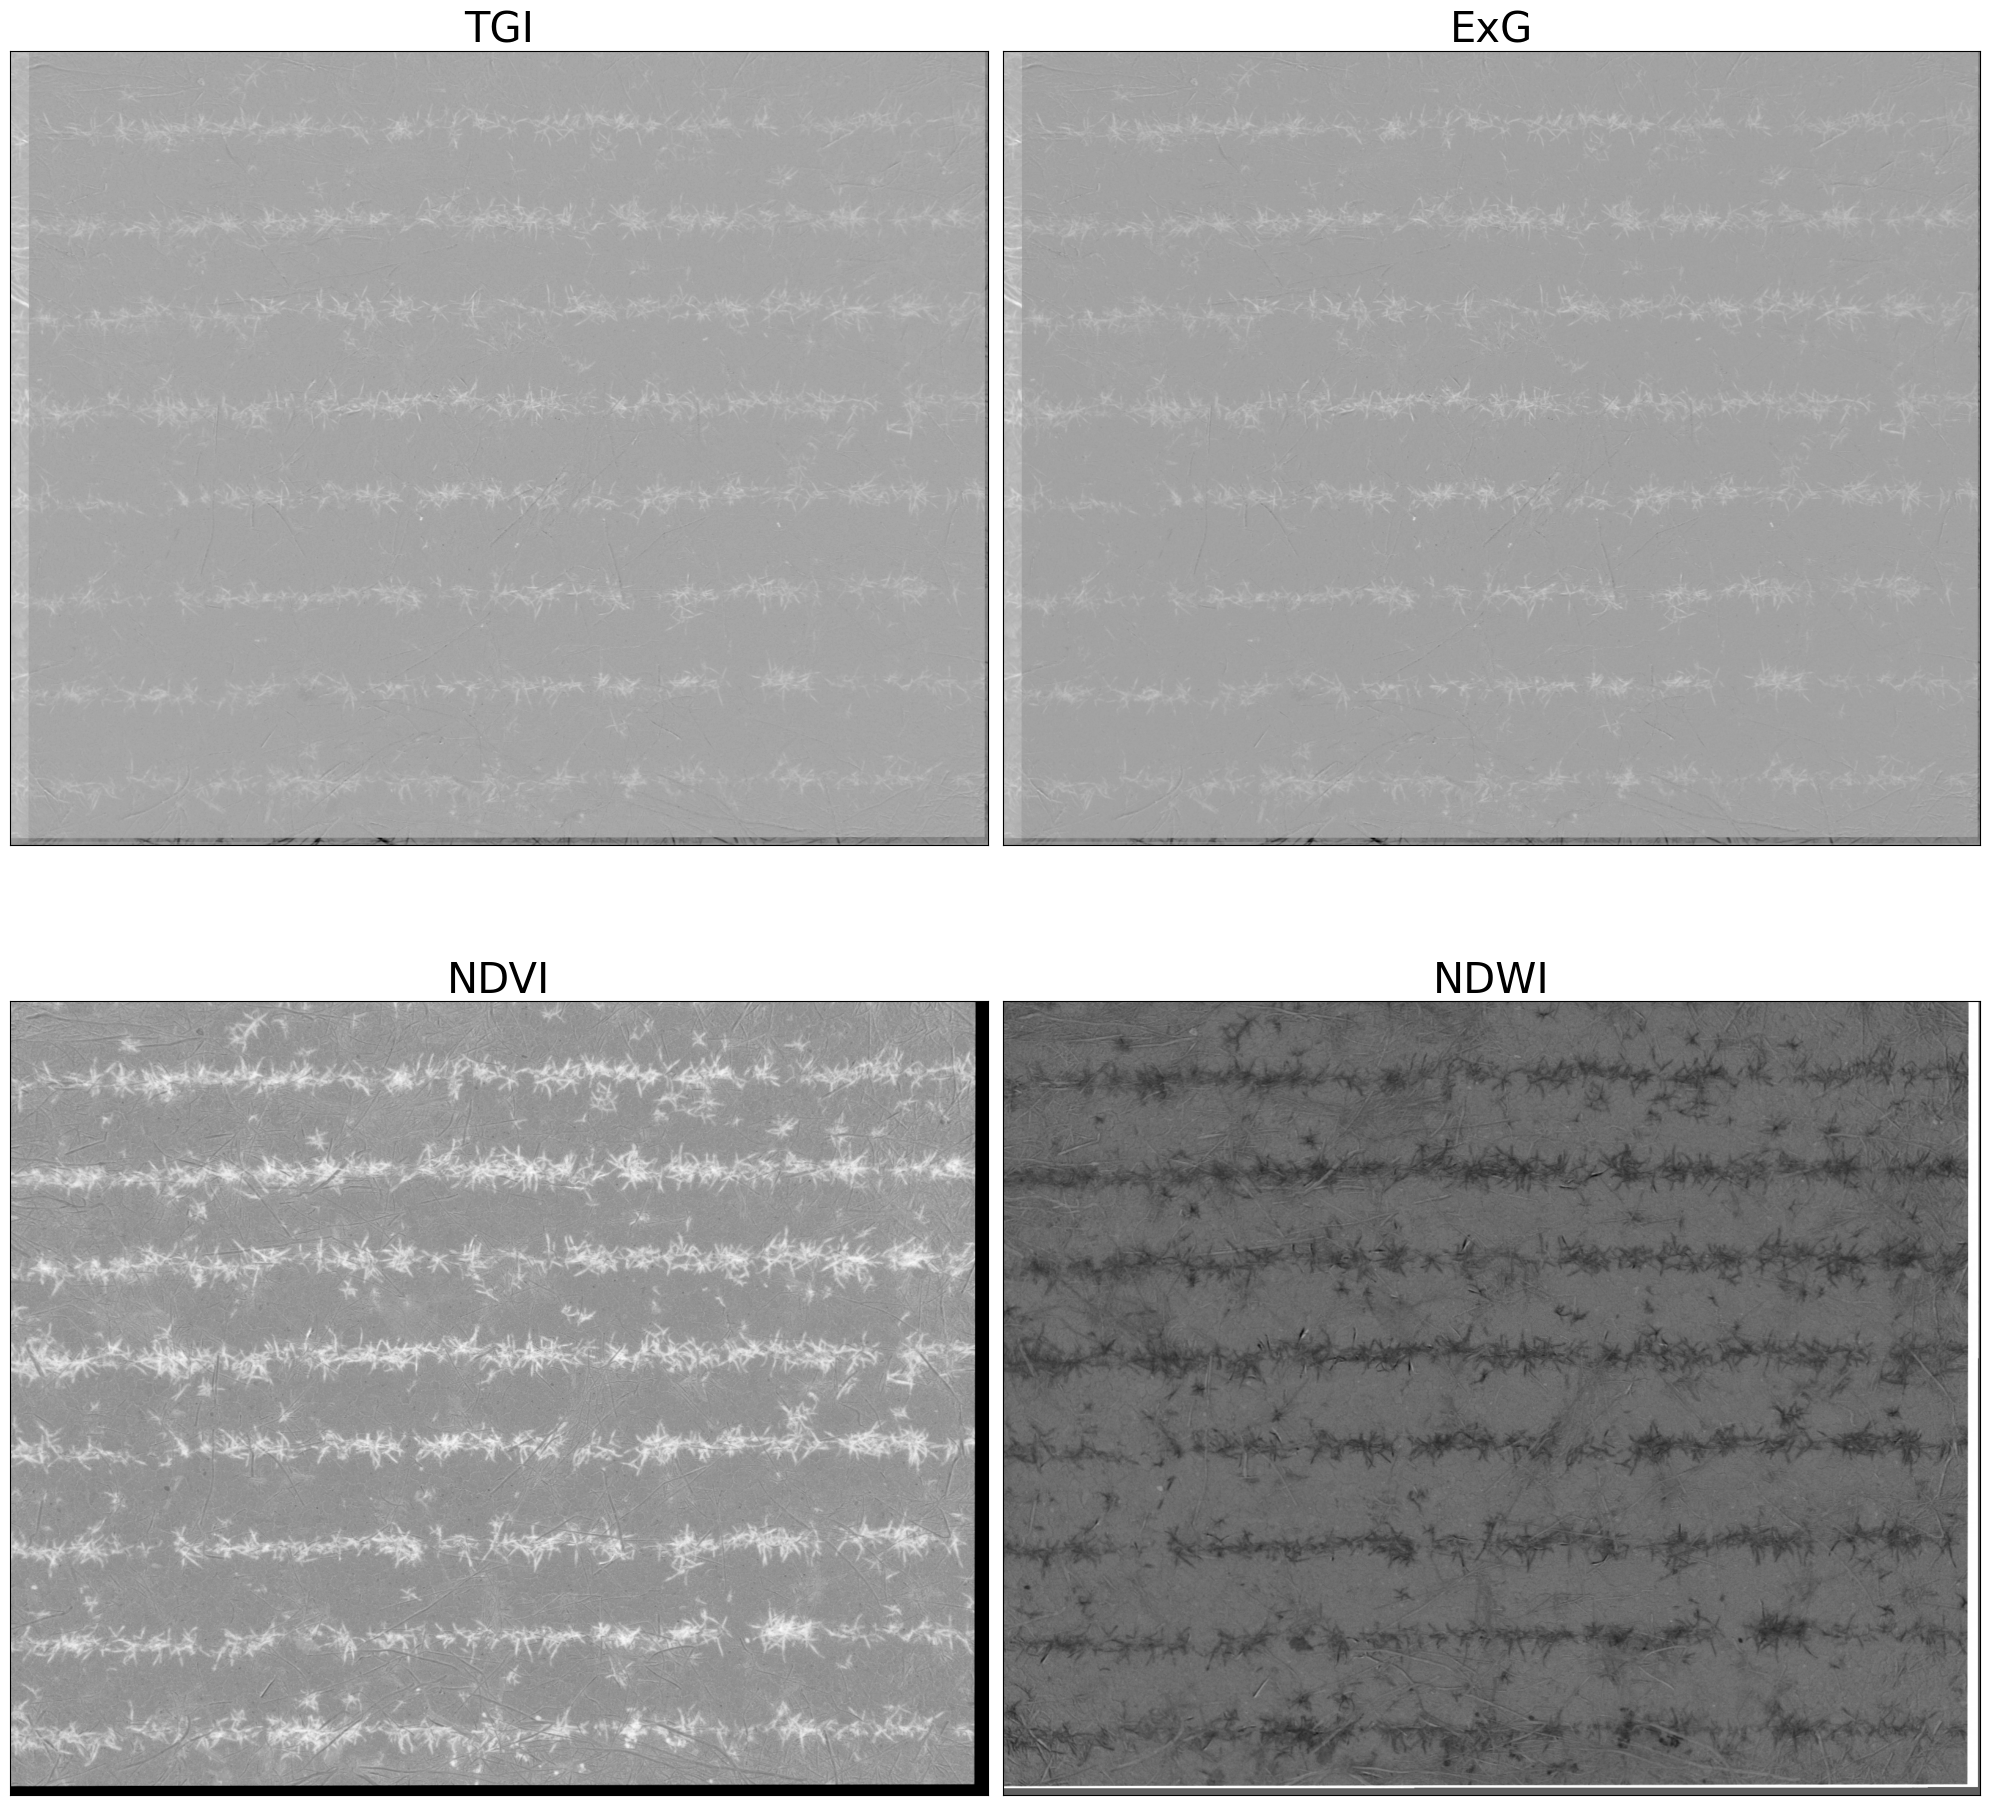
\includegraphics[width=0.95\textwidth]{images/VI_images_no_colorbar.png}
\caption{Qualitative visualization of the vegetation-index images used in the study. The four panels show the same aligned field scene transformed into TGI, ExG, NDVI, and NDWI views. Each panel is normalized for display, so the figure should be interpreted as a visual comparison of spatial patterns rather than as an axis-based or quantitatively scaled measurement of vegetation-index values.}
    \label{fig:VI-Images}
\end{figure*}

Figure~\ref{fig:VI-Images} illustrates that TGI, NDVI, and ExG emphasize green vegetation differently from NDWI in this scene. TGI and ExG emphasize visible greenness, while NDVI uses the contrast between NIR and red reflectance. NDWI was originally designed around green and NIR reflectance and therefore behaves differently for vegetation-dominated pixels. In this study, the figure is used to show qualitative differences among candidate input channels, not to compare absolute VI magnitudes across panels.

\subsection{Model and Training Adaptation}

The detector is based on a YOLO instance-segmentation architecture \cite{Jocher_Ultralytics_YOLO_2023}, adapted to accept multispectral inputs.\footnote{The reported experiments were implemented with Ultralytics YOLOv8-seg. The article refers to the detector more generally as YOLO-based because the contribution is the multispectral input adaptation and VI-channel comparison rather than a version-specific change to the model family.} In contrast to conventional YOLO networks that use RGB images, the baseline configuration uses the five aligned spectral bands captured by the UAV (Blue, Green, Red, Red Edge, and Near-Infrared (NIR); see Section~\ref{seq:VI}). The architecture-level adaptation is the input-channel configuration: the baseline uses five input channels, while the VI configurations use six input channels. The backbone and segmentation head follow the standard YOLO segmentation design; no new detection block is introduced.

As previous studies have also confirmed, multispectral data can improve detection in agricultural settings by providing spectral information beyond the visible range \cite{liu_automated_2023, sportelli_evaluation_2023, dutta_multispectral_2021, tang_cgs_yolo_2025}. We therefore evaluate whether adding a single vegetation-index (VI) channel to the five-band baseline improves black-grass detection.

The investigated input-channel configurations are compared to a baseline \emph{5-channel} configuration (five spectral bands only) and to otherwise identical 6-channel configurations where the same five bands are supplemented with one additional VI channel (NDVI, TGI, ExG, or NDWI). This controlled design analyzes the impact of each vegetation index separately while avoiding a comparison across different detector families.

The training loop was adapted to use stacked multispectral arrays rather than RGB images. Because hue-, saturation-, and value-based color augmentation assumes RGB-like image semantics and is not directly meaningful for stacked spectral bands and VI channels, the HSV augmentation terms were disabled in the multispectral training runs. Geometric augmentations and other training settings were handled within the YOLO training framework.

Precise band-to-band alignment is crucial for both vegetation-index computation and reliable training and inference. Accordingly, all spectral bands were geometrically aligned before stacking the channels and feeding them to the network (Figure~\ref{fig:Model-graph}).

\begin{figure*}[t]
    \centering
    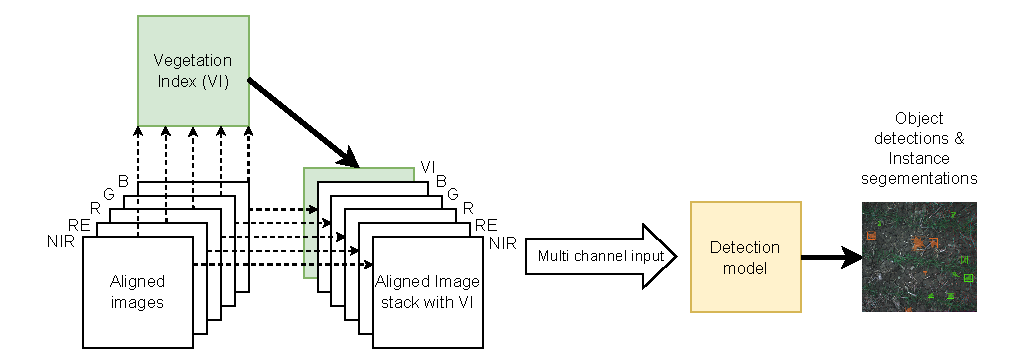
\includegraphics[width=0.95\textwidth]{images/Model Black-grass yolo v2.drawio.pdf}
    \caption{Data-processing pipeline for detecting black-grass. Five aligned multispectral bands (Section~\ref{seq:VI}) are stacked together with an optional vegetation-index channel to form the YOLO segmentation input used for both training and inference. The baseline (5-channel) configuration uses only the aligned bands as input, while each 6-channel configuration adds one vegetation-index channel.}
    \label{fig:Model-graph}
\end{figure*}

\begin{table}[t]
\centering
\caption{Reproducibility details for the controlled detector comparison.}
\label{tab:reproducibility_details}
\scriptsize
\begin{tabular}{p{0.29\linewidth} p{0.55\linewidth}}
\toprule
\textbf{Item} & \textbf{Description} \\
\midrule
Detector family & YOLO instance segmentation with the standard YOLO segmentation backbone and head. \\
Implementation & Ultralytics YOLO training with CUDA acceleration configured in the training script; see the method footnote for the implementation version. \\
Input configurations & 5-channel baseline (B, G, R, RE, NIR) and 6-channel VI configurations (B, G, R, RE, NIR plus one of TGI, ExG, NDVI, or NDWI). \\
Training data unit & One aligned UAV image stack from a single drone capture position and its corresponding YOLO segmentation annotation file. The reported detector study did not use a field-scale orthomosaic that was later tiled into smaller detector samples. \\
Acquisition sessions used in the reported study & All reported training, validation, and test data in this article were restricted to selected acquisition sessions within the observability window. \\
Data split & Train, validation, and test samples were assigned from different field zones. Within the final dataset preparation, annotated image/label files were split into 70\% training, 15\% validation, and 15\% test data. \\
Multispectral training adaptation & The training pipeline used stacked multispectral arrays instead of RGB images. RGB-specific HSV augmentation terms were disabled for the multispectral runs. \\
Evaluation thresholds & The PR and F1-confidence curves sweep the detector confidence score rather than reporting one fixed operating threshold. AP is computed from the resulting PR behavior after matching predicted and annotated instances. \\
Bootstrap confidence intervals & Table~\ref{tab:performance_metrics_by_position} reports 95\% CIs from a detection-level nonparametric bootstrap. Matched detection outcomes and detector confidence scores were resampled with replacement 10{,}000 times; AP was recomputed for each resample and CIs are percentile intervals. \\
\bottomrule
\end{tabular}
\end{table}

\section{Experiment}

\subsection{Data Acquisition}
The broader acquisition campaign covered two winter wheat fields in the south of Sweden. In each field, we had a designated parcel of approximately 20~m $\times$ 20~m. The parcels had a recorded occurrence of black-grass. The campaign imagery was reviewed across the growing season to identify the period where black-grass could be annotated reliably and where detection would be agronomically useful.

We distinguish between two related but separate timing concepts. In this study, the \emph{observability window} denotes the approximately two- to three-week spring period in which black-grass in the examined winter-wheat fields was sufficiently developed to be visually or spectrally distinguished from wheat, but before wheat growth caused strong occlusion. The \emph{susceptibility window} denotes the partly overlapping period in which chemical control of black-grass remains biologically and operationally relevant. These windows should be understood as phenological and field-condition-dependent rather than fixed calendar periods: in milder or colder seasons, the same practical window may shift earlier or later depending on local weather, crop development, and weed growth stage. The distinction is important because herbicide efficacy for black-grass is growth-stage dependent; for example, Pintar et al. reported substantially reduced pinoxaden efficacy when applications were delayed to later growth stages \cite{pintar_growth_stage_2021}. In Swedish winter-wheat practice, local recommendations likewise frame selective treatment as stage limited rather than universally available throughout the season \cite{renkavle}.

The data was collected using a multispectral drone, equipped with five single-band cameras with 2-megapixel (2~MP) sensors: Blue (B), Green (G), Red (R), Red Edge (RE), and Near-Infrared (NIR). The drone was flown at a speed of 1~m/s and altitudes of 1-2~meters, capturing images with a resolution of 0.6-1.2~mm/pixel and consequently an area of 0.8~m $\times$ 1.0~m to 1.6~m $\times$ 2.0~m. 

The detector dataset used in the reported experiments was restricted to the selected acquisition sessions on 27~March~2023 and 12~April~2023 across the study fields. No data from earlier or later flights were included in the reported training, validation, or test splits. These two sessions were selected because they fell within the practical overlap between the observability window and the susceptibility window in the studied fields: the wheat had not yet grown over the black-grass plants, while the black-grass had developed enough to be visually and spectrally differentiated from wheat during annotation. Earlier flights were less useful because the target plants were harder to distinguish, while later flights suffered from increasing crop occlusion and were less aligned with the intended early-season control context.

The topography of the parcels featured stiff clay soil interspersed with debris from the previous year's harvest, producing bright residue and background structures that complicated visual interpretation in both RGB and VI views, see Figures~\ref{fig:VI-Images} and \ref{fig:comparison}. Wheat was sown in rows spaced 25~cm apart, and images were oriented to capture these rows horizontally, thus maintaining consistency in the viewing angle and direction across all datasets.

\subsection{Annotation}
The data annotation process was critical for preparing the images for training and evaluating the detector for weed detection. The annotations were conducted using both RGB and NDVI images as references, with human experts carefully reviewing the images to identify and mark the positions of black-grass.

A single experienced annotator performed all annotations, ensuring consistency across the dataset. This annotator was well-versed in recognizing the specific visual characteristics of black-grass and wheat, which can be particularly challenging during their early growth stages when they appear visually similar. To address this challenge, the annotator used NDVI images alongside RGB images. The NDVI images provided additional spectral information that highlighted differences in vegetation health, aiding in the accurate identification of black-grass.

The NDVI images were used as a visual support source during annotation, not as an automatic labeling rule. Because NDVI was also evaluated as one of the model input channels, this annotation support is an important validity consideration: NDVI-assisted annotation may influence interpretation of the NDVI-channel results. We therefore interpret the NDVI configuration cautiously and focus the main conclusions on the comparative behavior across all VI configurations rather than treating NDVI as a fully independent annotation-free signal.

The resulting annotated data included labels specifying the presence of black-grass and its positional relationship to the wheat rows (either within the rows or between the rows).

\subsection{Image Alignment}
As mentioned earlier, the alignment of multispectral images is critical for ensuring that different spectral bands are precisely overlaid for subsequent analysis \cite{pettorelli2013}. The process was done for all the images in the dataset. The alignment also facilitated the computation of the VIs. 

The first step in this process is sensor calibration to remove radial and tangential distortions from multispectral images. Radial distortion results from the lens's shape, whereas tangential distortion is due to imperfection in the lens assembly for each multispectral camera \cite{bradski2008learning}. To correct these distortions, a set of coefficients was computed and applied to the original image coordinates.

After calibration, keypoints are detected and matched across images using the Scale-Invariant Feature Transform (SIFT) \cite{lowe2004}. SIFT detects keypoints and computes descriptors that are invariant to image scaling, translation, rotation, and partially invariant to changes in illumination and affine or 3D projection. Keypoints between images are matched using the nearest neighbor approach in the feature space, followed by a ratio test to refine the matches \cite{muja2009}.

The matched keypoints are then used to compute a transformation matrix that best aligns the two images. This matrix is calculated using a method that minimizes the back-projection error, ensuring that the transformed points in one image match as closely as possible to their corresponding points in the other image \cite{hartley2003}. This process ensures that multispectral images are overlaid precisely, which is fundamental for computing vegetation indices \cite{hallosta_multispectral_2024}. For example, the NDVI is computed using the NIR and red images through this process.

\subsection{Dataset Construction and Split}
The final detector dataset was constructed from aligned multispectral image stacks and their corresponding segmentation annotations. Each training or evaluation sample corresponds to one drone capture position represented by one aligned UAV image stack built from the five spectral bands. The reported detector study did not first generate a field-scale orthomosaic and then tile it into detector patches; instead, the aligned image stacks themselves formed the candidate sample units. No additional overlapping patch-generation step was applied after this stack-generation stage for the reported experiments.

Only image stacks from the selected observability-window sessions that could be annotated reliably were retained for the detector comparison. No image stacks from earlier or later flights were included in the reported detector dataset. The final split was designed so that training, validation, and test samples came from different parts of the field. Within this dataset preparation, the annotated image/label files were split into 70\% training, 15\% validation, and 15\% test data.

This split reduces direct reuse of the same image content across training and evaluation, but it does not remove all possible leakage-like effects. The subsets still come from the same field, acquisition setup, soil background, and narrow crop-growth window. The results should therefore be interpreted as a controlled within-field evaluation of VI-channel effects, not as proof of full geographic or seasonal generalization.

\section{Results}
Our analysis investigates how different vegetation indices influence the network's ability to detect black-grass.
The primary indices considered were the Triangular Greenness Index (TGI), Excess Green Index (ExG), Normalized Difference Vegetation Index (NDVI), and Normalized Difference Water Index (NDWI). These indices were assessed using performance metrics, including average precision (AP), recall, and F1-score. In line with previous studies \cite{su_spectral_2022}, the TGI index shows strong performance on several metrics, indicating that it can enhance detection performance for some operating points.

In the PR and F1-confidence analyses, the threshold refers to the confidence score assigned by the detector to each predicted instance. The curves therefore show how precision, recall, and F1-score change as this confidence threshold is swept, rather than reporting performance at a single fixed threshold.

\begin{figure*}[htbp]
    \centering
    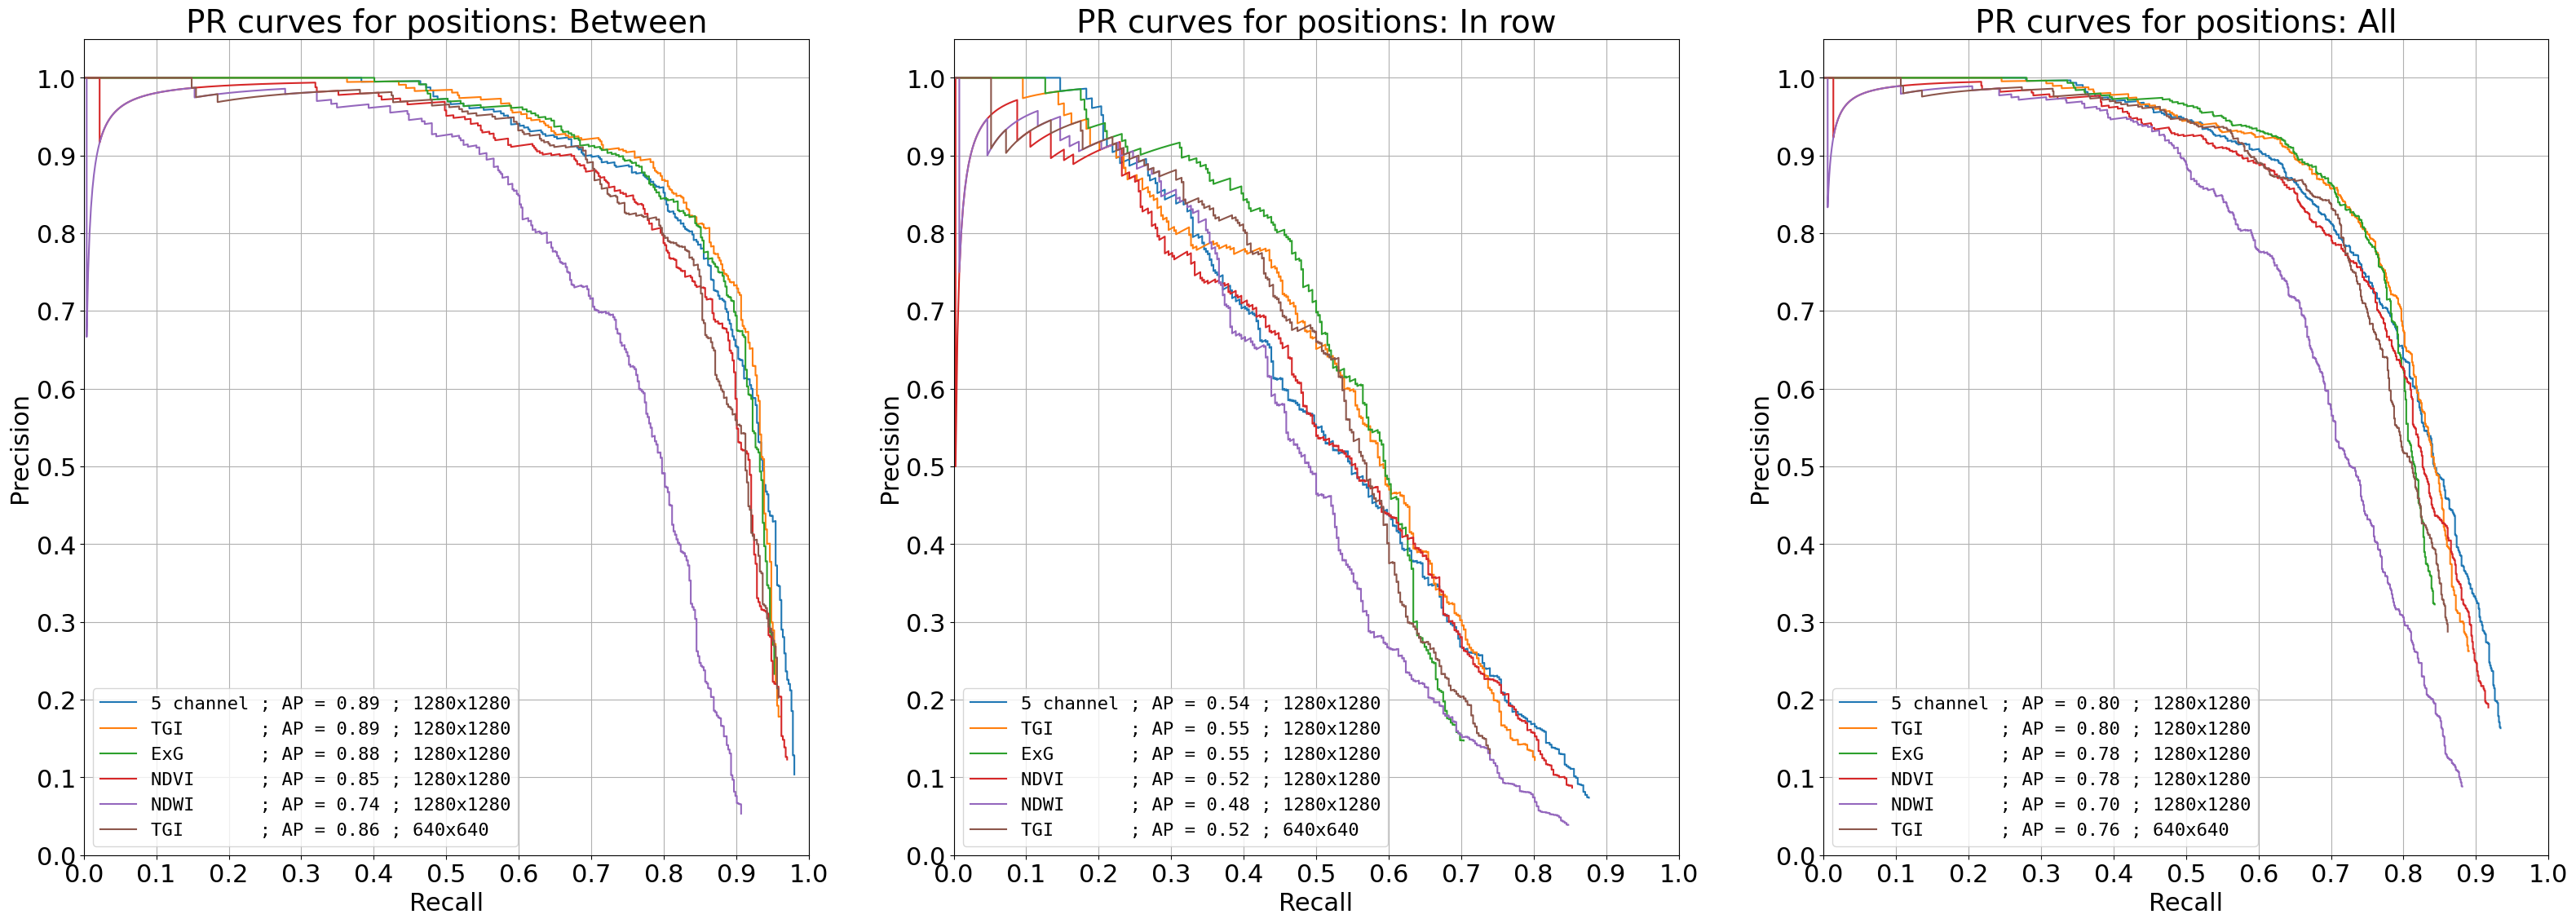
\includegraphics[width=1\textwidth]{images/PR-curves_Different_Positions_v3.png}
    \caption{Precision--recall (PR) curves for different input-channel configurations across three positional categories: Between, In row, and All. The configurations evaluated are the 5-channel baseline and the TGI, ExG, NDVI, and NDWI configurations at 1280$\times$1280 resolution, plus one additional TGI probe at 640$\times$640. The PR curves illustrate the trade-off between precision and recall as detector confidence scores are swept.}
    \label{fig:PR-curves-positions}
\end{figure*}

\subsection{Precision--recall characteristics across confidence thresholds}
As illustrated in Figure~\ref{fig:PR-curves-positions}, the precision--recall (PR) curves show that the Triangular Greenness Index (TGI) and Excess Green Index (ExG) configurations maintain higher precision over substantial parts of the recall range in the evaluated field data. This suggests that these VI channels can help distinguish black-grass from wheat under the reported acquisition conditions. The effect is clearest between rows, while all configurations remain more challenged in-row because wheat occlusion and weed--crop similarity are higher. The baseline 5-channel configuration reaches high recall at lower confidence thresholds, but with lower precision in parts of the sweep. This trade-off is further emphasized in the F1-score curves shown in Figure~\ref{fig:F1-curves-positions}.

\subsection{Average Precision (AP) and confidence intervals (CIs)}
To provide a threshold-aggregated summary of detection performance, we report Average Precision (AP) \cite{lin_coco_2014} together with 95\% confidence intervals (CIs) from a detection-level nonparametric bootstrap \cite{efron1979bootstrap}.
For each input-channel configuration and positional subset, predictions were first matched to annotated instances using the same matching procedure used for the PR analysis. The matched detection outcomes and detector confidence scores were resampled with replacement 10{,}000 times. For each bootstrap resample, the PR curve and AP were recomputed, and the 95\% CI was defined by the 2.5th and 97.5th percentiles of the resulting AP distribution.
For completeness, we also report results for a TGI configuration trained at a reduced input resolution (640$\times$640), whereas the remaining configurations were trained and evaluated at 1280$\times$1280.
Table~\ref{tab:performance_metrics_by_position} presents the AP values and their 95\% confidence intervals for each configuration and positional category. Key observations include:
\begin{itemize}
    \item \textbf{Between Rows:} The TGI configuration achieves the highest AP (0.892), closely followed by the 5-channel baseline (0.889). The NDWI configuration underperforms with an AP of 0.742.
    \item \textbf{In Rows:} All configurations show reduced performance due to occlusion by wheat. The TGI configuration maintains a relatively higher performance (AP~=~0.553), closely followed by ExG (AP~=~0.547), \mbox{5-channel (AP~=~0.545)} and NDVI (AP~=~0.523).
    \item \textbf{All:} The 5-channel baseline achieves the highest AP of 0.805, followed by the TGI configuration (1280$\times$1280) with an AP of 0.800. While the baseline is marginally higher on the combined set, the TGI configuration performs comparatively better when the data are analyzed separately by positional category, suggesting that the overall ranking is influenced by the composition of the combined dataset.
\end{itemize}

\begin{table}[htbp]
\centering
\caption{Average Precision (AP) values for each input-channel configuration and position, along with their corresponding 95\% confidence intervals from the detection-level 10{,}000-resample bootstrap analysis.}
\begin{tabular}{lll}
\toprule
\multicolumn{1}{c}{\textbf{Configuration}} & \multicolumn{1}{c}{\textbf{AP}} & \multicolumn{1}{c}{\textbf{95\% CI}} \\
\midrule
\multicolumn{3}{c}{\textbf{Position: Between}} \\
5-channel 1280$\times$1280 & 0.889 & (0.810 - 0.971) \\
\textbf{TGI 1280$\times$1280} & \textbf{0.892} & \textbf{(0.812 - 0.970)} \\
ExG 1280$\times$1280 & 0.884 & (0.808 - 0.959) \\
NDVI 1280$\times$1280 & 0.855 & (0.773 - 0.935) \\
NDWI 1280$\times$1280 & 0.742 & (0.660 - 0.823) \\
TGI 640$\times$640 & 0.856 & (0.776 - 0.933) \\
\midrule
\multicolumn{3}{c}{\textbf{Position: In rows}} \\
5-channel 1280$\times$1280 & 0.545 & (0.467 - 0.625) \\
\textbf{TGI 1280$\times$1280} & \textbf{0.553} & \textbf{(0.473 - 0.635)} \\
ExG 1280$\times$1280 & 0.547 & (0.472 - 0.625) \\
NDVI 1280$\times$1280 & 0.523 & (0.440 - 0.607) \\
NDWI 1280$\times$1280 & 0.483 & (0.405 - 0.561) \\
TGI 640$\times$640 & 0.525 & (0.447 - 0.603) \\
\midrule
\multicolumn{3}{c}{\textbf{Position: All}} \\
\textbf{5-channel 1280$\times$1280} & \textbf{0.805} & \textbf{(0.748 - 0.865)} \\
TGI 1280$\times$1280 & 0.800 & (0.746 - 0.854) \\
ExG 1280$\times$1280 & 0.778 & (0.728 - 0.829) \\
NDVI 1280$\times$1280 & 0.783 & (0.727 - 0.840) \\
NDWI 1280$\times$1280 & 0.696 & (0.640 - 0.754) \\
TGI 640$\times$640 & 0.765 & (0.711 - 0.818) \\
\bottomrule
\end{tabular}
\label{tab:performance_metrics_by_position}
\end{table}

\begin{figure*}[htbp]
    \centering
    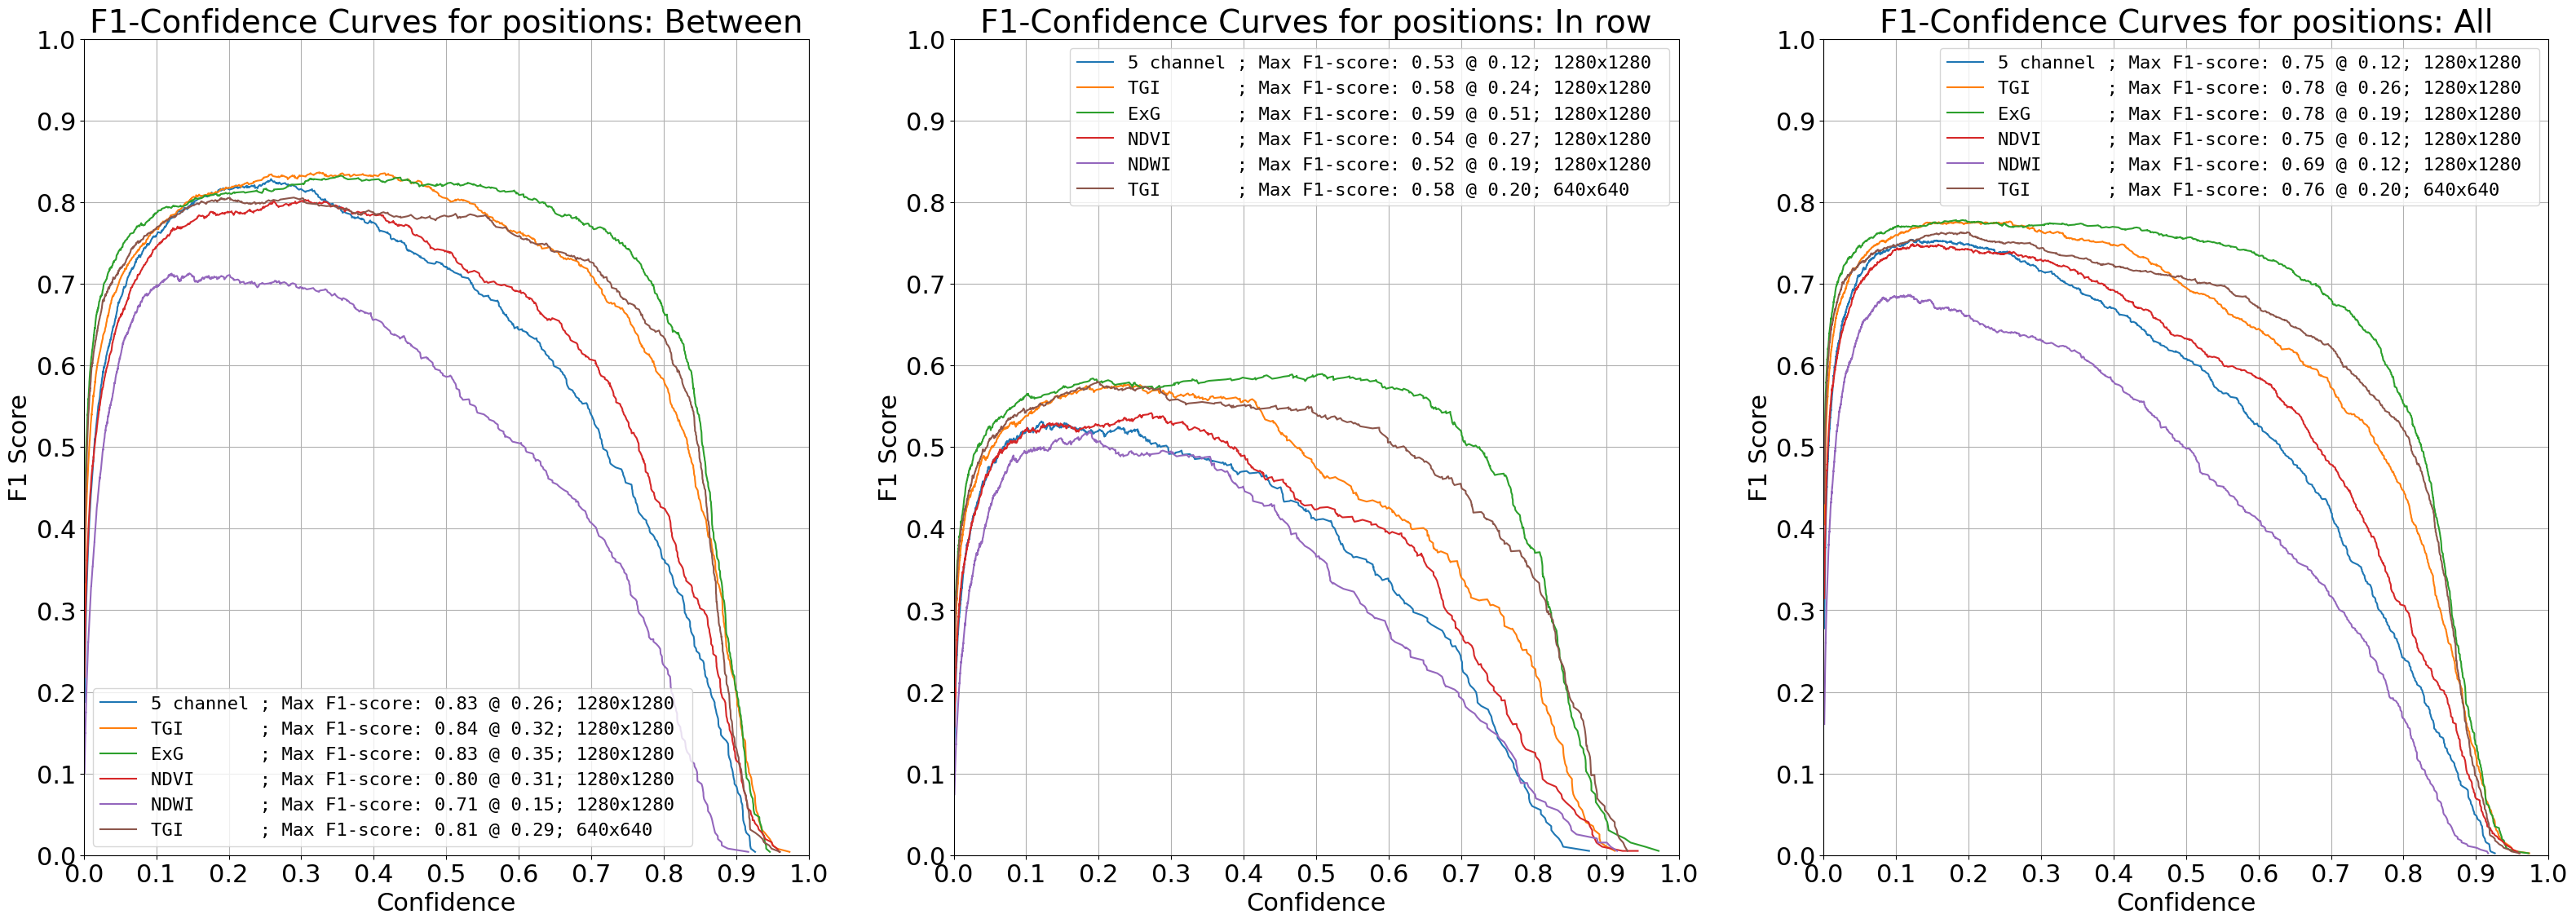
\includegraphics[width=1\textwidth]{images/F1-Confidence-curves_Different_Positions_v3.png}
    \caption{F1-confidence curves for different input-channel configurations across three positional categories: Between, In row, and All. The configurations evaluated include the 5-channel baseline and the TGI, ExG, NDVI, and NDWI configurations at 1280$\times$1280 resolution, plus one additional TGI probe at 640$\times$640. The F1 score represents the harmonic mean of precision and recall as a function of detector confidence score.}
    \label{fig:F1-curves-positions}
\end{figure*}

Figures~\ref{fig:PR-curves-positions} and \ref{fig:F1-curves-positions} depict PR behavior and F1-confidence curves, respectively. Together, these curves highlight the precision--recall trade-off when selecting confidence thresholds for practical deployment. In particular, the TGI and ExG configurations tend to achieve more balanced performance across thresholds, whereas the baseline 5-channel configuration reaches high recall at the cost of lower precision at lower confidence thresholds.

The detailed analysis reveals several key insights:
\begin{itemize}
    \item \textbf{Configuration Performance:} The additional TGI run at lower resolution (640$\times$640) remains competitive with some 1280$\times$1280 configurations, but it should be interpreted only as a targeted probe because equivalent lower-resolution runs were not available for the other VIs.
    \item \textbf{Positional Differences:} There is a notable difference in detection performance between weeds located between rows and those within rows, with better performance in less occluded conditions. This underscores the need for robust detection under occlusion.
\end{itemize}

The bootstrap confidence intervals quantify uncertainty in the AP estimates under this matched detection-outcome resampling scheme, not variation across new fields or seasons.

\section{Discussion}
Our study investigates the impact of different vegetation indices on the performance of neural networks in detecting black-grass using UAV-acquired multispectral images. The main findings are as follows:

\begin{itemize}
    \item The TGI index demonstrated the strongest AP in the between-row and in-row categories, closely followed by the ExG index, while the 5-channel baseline remained strongest in the combined AP summary.
    \item The NDWI index underperformed compared to the other indices, negatively impacting the detector's performance in this configuration.
    \item The targeted TGI 640$\times$640 probe remained competitive with some 1280$\times$1280 configurations, but the study does not establish a general resolution trend across all VIs.
    \item The 5-channel baseline configuration achieved the highest overall recall.
\end{itemize}

\subsection{Configuration Performance and Interpretation}
The favorable behavior of the TGI and ExG configurations is likely related to how these indices preserve visible greenness differences between black-grass and wheat in the reported scenes. This interpretation is consistent with the results of Su et al., who found that specific vegetation indices can improve the accuracy of black-grass weed mapping models \cite{su_spectral_2022}. It also aligns with recent black-grass studies showing that multispectral and hyperspectral cues are informative in cereal crops, while also being sensitive to acquisition setting and between-site variation \cite{cox_black-grass_2023, goodsell_black_grass_2024, darbyshire_blackgrass_2025}.

The comparison with Darbyshire et al.~\cite{darbyshire_blackgrass_2025} is most informative when viewed through the evaluation task rather than the headline score. Their reported 89.6\% image-level classification accuracy and the between-row AP of 0.892 for our TGI configuration are numerically similar, but they measure different errors: classification can succeed by assigning the correct class to an image, whereas instance segmentation requires individual black-grass instances to be localized with sufficient overlap and confidence. The lower in-row AP (0.553 for TGI) therefore suggests that the harder part of the present problem is not only recognizing a black-grass spectral signature, but preserving instance-level localization under wheat occlusion and crop--weed similarity.

In contrast, the NDWI configuration appears less aligned with the spectral cues that separated black-grass from wheat in this dataset. This weaker behavior should be interpreted in the context of site-specific spectral conditions, since previous work has shown that weed-mapping performance can vary with environmental conditions and acquisition setting \cite{lambert_evaluating_2018}.

The 5-channel baseline configuration achieved the highest recall, indicating its effectiveness in detecting most occurrences of black-grass. However, the TGI and ExG configurations maintained higher precision, providing more reliable detections with fewer false positives. This trade-off is crucial depending on the application--whether the goal is to detect all weeds or to ensure precise detection with minimal errors.

\subsection{Detection Between and In Rows}
An essential aspect of our findings is the difference in detection performance between rows and within rows of wheat. Figures~\ref{fig:PR-curves-positions} and \ref{fig:F1-curves-positions}, along with Table \ref{tab:performance_metrics_by_position}, show that the configurations are more successful in identifying black-grass between rows, where there is less occlusion and higher contrast. In-row detection is hindered by occlusion and visual similarity between wheat and black-grass, leading to lower precision and recall. For instance, the TGI configuration achieved an AP of 0.892 between rows compared to 0.553 within rows. This highlights the need for advanced techniques to improve in-row detection, which remains a significant challenge for UAV-based weed detection.

\begin{figure*}[h]%[htbp]
    \centering
    \subfigure[Original RGB image]{%
        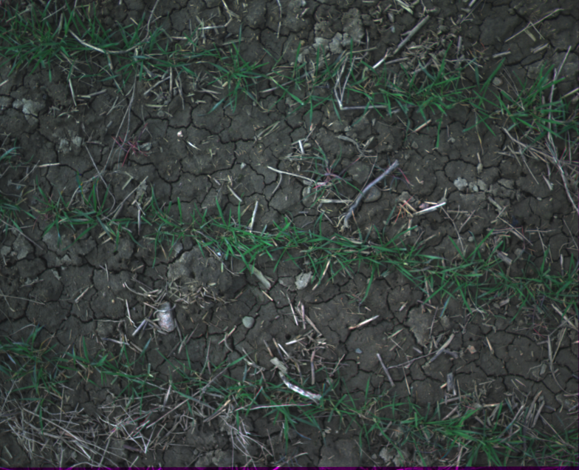
\includegraphics[width=0.3\textwidth]{images/Original-RGB.png}
    }\hfill
    \subfigure[Predictions in RGB image]{%
        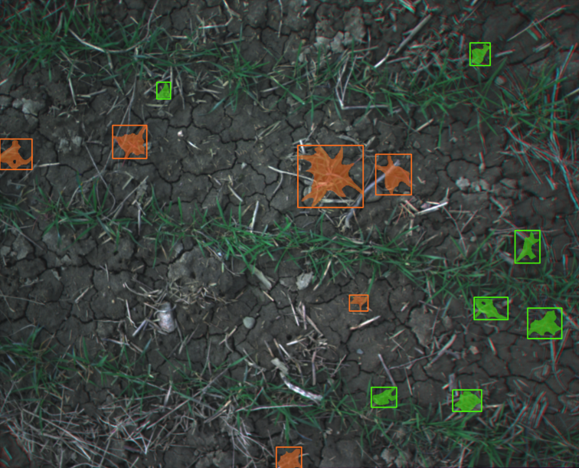
\includegraphics[width=0.3\textwidth]{images/Predictions-rgb.png}
    }\hfill
    \subfigure[Annotations in NDVI image]{%
        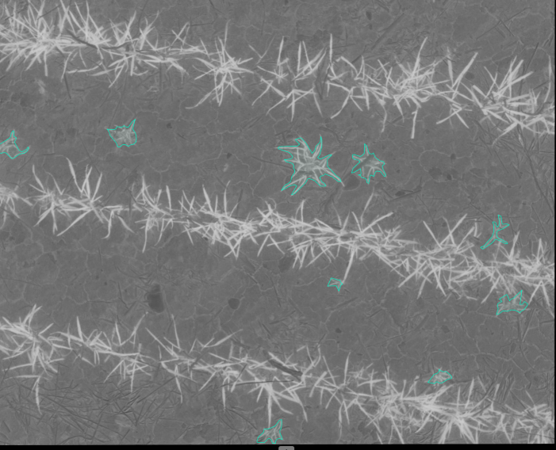
\includegraphics[width=0.3\textwidth]{images/Annotation-NDVI.png}
    }
    \caption{Qualitative comparison of the original RGB image (a), detector predictions shown on the RGB image (b), and annotations shown on the NDVI image used during labeling (c). Orange markings indicate black-grass classified as between rows, while green masks indicate black-grass located in the wheat rows. The detector used for predictions is the reference 5-channel configuration trained on the original five image bands.}
    \label{fig:comparison}
\end{figure*}

\subsection{Qualitative Interpretation of Predictions and Annotations}

Figure~\ref{fig:comparison} compares the original RGB view, detector predictions, and the NDVI-assisted annotation view for the same scene. The example shows that some predicted regions occur near visually ambiguous vegetation structures. These cases are useful for understanding detector--annotation disagreement, but they should not be treated as confirmed annotation errors without additional field validation. The qualitative example therefore supports a cautious interpretation of false positives rather than a claim that precision is systematically underestimated.



\subsection{Practical Implications}
The findings of this study have significant implications for precision agriculture:

\begin{itemize}
    \item UAVs equipped with multispectral cameras and carefully selected VI-channel configurations could support more precise weed-localization workflows during the overlap between the observability and susceptibility windows. Lambert et al. emphasized the importance of high-resolution imagery and advanced modeling techniques in enhancing weed management practices \cite{lambert_testing_2019}. Recent UAV-based deep-learning work also shows how detector outputs can support site-specific weed-management products such as treatment maps, although such map generation is beyond the scope of the present study \cite{mesias_ruiz_multispecies_2026}. Related patent literature has also described multispectral image mapping and convolutional-neural-network detection for identifying weeds such as black-grass in winter wheat \cite{hallosta_weed_patent_2025}.
    \item Selecting an appropriate vegetation-index input can improve the precision--recall trade-off for black-grass detection in the reported setup. Translation into operational herbicide reduction requires additional field-scale validation and treatment-map integration.
\end{itemize}

\subsection{Challenges and Limitations}
Several challenges were encountered during the study:

\begin{itemize}
    \item \textbf{Timing Window:} The reported detector experiments used only selected acquisition sessions within the most useful overlap between the observability and susceptibility windows in the studied fields. This was the period when visual separation between black-grass and wheat was sufficient and before wheat growth caused strong occlusion of black-grass. The exact calendar timing should not be generalized directly across years or regions because both crop and weed development depend on local weather and phenological conditions.
    \item \textbf{Image Alignment:} Accurate alignment of multispectral images is crucial. Misalignment can significantly degrade the quality of vegetation indices and the subsequent analysis. Robustness to alignment errors and different sensor conditions was not evaluated separately in this study.
    \item \textbf{Within-field Evaluation:} The train, validation, and test subsets were drawn from different parts of the same field and from a narrow acquisition window. This supports a controlled comparison of VI-channel effects under similar field conditions, but it may also simplify the generalization problem and should not be interpreted as a fully independent field-level generalization test.
    \item \textbf{NDVI-assisted Annotation:} NDVI was used as visual support during annotation. This may affect interpretation of the NDVI input-channel configuration and motivates cautious conclusions about NDVI-specific performance.
    \item \textbf{Small Sample Size:} The study's sample size is limited. Increasing the dataset size across various fields and seasons would enhance the generalizability of the results.
\end{itemize}

These challenges are consistent with those reported by Lambert et al., who noted the importance of precise image alignment and the potential limitations posed by small sample sizes in UAV-based studies \cite{lambert_evaluating_2018}.

\subsection{Technical Insights}
The alignment and calibration of multispectral images were crucial steps for producing coherent VI channels and detector inputs. Because the reported comparison keeps the detector family fixed and varies the VI channel, the results should be interpreted as evidence about input-channel choice rather than as evidence for a new detector architecture. Future studies should preserve fuller training logs and runtime metadata so that convergence behavior and computational cost can be evaluated more directly.


\subsection{Future Research Directions}
Future research should explore additional vegetation indices and their combinations to further improve weed detection models. Investigating the integration of synthetic data for training models can also address data scarcity and improve model robustness. Additionally, expanding the study to include diverse geographic locations and different crop types would provide a broader understanding of the applicability of these techniques.

\section{Conclusion}

This study examined how adding a single vegetation-index channel affects black-grass detection with a fixed YOLO instance-segmentation detector family and multispectral UAV input. The TGI and ExG configurations improved the precision-oriented operating behavior in important parts of the evaluation, while the 5-channel baseline remained competitive and achieved the highest AP in the combined summary.

These results underline the potential of UAV-acquired multispectral imagery and VI-channel selection for black-grass detection, while also showing that the benefit is context dependent. The strongest gains were observed for between-row and in-row positional analyses, whereas broader operational claims require validation across additional fields, seasons, and management workflows.

Further research should explore the combination of additional vegetation indices, improve detection in occluded environments, and expand the study to include other crop types and regions, thereby enhancing the applicability of these techniques in diverse agricultural settings.


\section{ACKNOWLEDGMENT}
The authors would like to express their sincere gratitude to Marcus Willert (HIR) for his expertise in black-grass identification and guidance on agricultural practices, Jan Jönsson (Ly-Ros) for providing the farmland necessary for this study, and Jonny Ulvtorp (JU Information) for his invaluable project management support. The authors also acknowledge the Municipality of Karlshamn and the Swedish Board of Agriculture for their financial support, which made this research possible. Special thanks are extended to Lena Nilsson for her meticulous work in annotating the data used for model training, which was crucial to the success of this project.

\bibliographystyle{IEEEtran}

\bibliography{IEEEabrv,IEEEexample}


\begin{IEEEbiography}[{
\includegraphics[width=1in,height=1.25in,clip,keepaspectratio]{images/Simon.png}}]{SIMON HALL\"OSTA}
received an M.Sc. degree in Engineering Mathematics, with a specialization in image analysis and machine learning, from Lund University, Sweden, in 2018, followed by the degree of Licentiate of Technology in Systems Engineering from Blekinge Institute of Technology, Karlskrona, Sweden, in 2025. He is currently pursuing a Ph.D. degree at Blekinge Institute of Technology.

His research focuses on artificial intelligence and multispectral imaging for precision agriculture, with an emphasis on UAV-based weed detection. The work has resulted in a pending patent and, in 2024, his research project was selected for the Royal Swedish Academy of Engineering Sciences' (IVA) 100 List, which highlights Swedish research with high potential for commercial and societal impact.
\end{IEEEbiography}



\begin{IEEEbiography}[{
\includegraphics[width=1in,height=1.25in,clip,keepaspectratio]{images/Saleh.PNG}}]{Saleh Javadi} (S'12-M’22) received a B.Sc. degree in electrical-control engineering from Amirkabir University of Technology in 2009, an M.Sc. degree in electrical, electronic, and systems engineering from the National University of Malaysia in 2013, and a Ph.D. degree in systems engineering from Blekinge Institute of Technology (BTH), Sweden, in 2021.

Saleh received the Innovator of the Year award in 2019 (SKAPA – Innovation Prize in Memory of Alfred Nobel) in Blekinge for innovative efforts in optimizing and reducing energy consumption in process industries using artificial intelligence. In addition, he was awarded the ÅForsk Entrepreneur’s prize by the Swedish Innovation Council in May 2019.

He is currently a Senior Lecturer at the Department of Mathematics and Natural Sciences at BTH. His research interests include signal processing, machine learning and computer vision.
\end{IEEEbiography}


\begin{IEEEbiography}[{
\includegraphics[width=1in,height=1.25in,clip,keepaspectratio]{images/Mattias.png}}]{MATTIAS DAHL} 
(Member, IEEE) received a B.Sc.~in Electrical Engineering from Chalmers University of Technology (1989), an M.Sc.~in Computer Science from Luleå University of Technology (1993), a Licentiate degree in Signal Processing from Lund University (1996), and a Ph.D.~in Applied Signal Processing from Blekinge Institute of Technology (2000). Since 2018, he has been a Full Professor at Blekinge Institute of Technology.
His research focuses on autonomous systems, smart sensor systems, applied artificial intelligence (AI), and sustainable engineering. He has led several national and EU-funded research programs and has played a key role in establishing marine technology testbeds, including novel underwater sensing solutions such as Distributed Acoustic Sensing (DAS). He has authored over 120 scientific publications, holds several patents (the latest filed in 2024), and has received innovation awards from Sweden’s Innovation Agency and the Royal Swedish Academy of Engineering Sciences (IVA).
Prof.~Dahl has supervised around 10 Ph.D.~students and is currently supervising three doctoral candidates. His work bridges academia and industry, with contributions in radar, vision, transport systems, and embedded sensing platforms.

\end{IEEEbiography}



\begin{IEEEbiography}[{
\includegraphics[width=1in,height=1.25in,clip,keepaspectratio]{images/Mats.png}}]{MATS I. PETTERSSON} 
(Senior Member, IEEE) received the M.Sc. in engineering physics, the licentiate degree in radio and space science, and the Ph.D.  in signal processing from the Chalmers University of Technology, Gothenburg, Sweden, in 1993, 1995, and 2000, respectively. 
He worked with Mobile Communication Research at Ericsson, Lund, Sweden. He was with the Swedish Defense Research Agency (FOI) for ten years in Linköping. He focused on ultrawideband low-frequency Synthetic Aperture Radar (SAR) systems at FOI. Since 2005, he has been with the Blekinge Institute of Technology (BTH), Karlskrona, Sweden, where he is a Full Professor. He has authored or co-authored more than 250 scientific publications, of which more than 70 are in peer-reviewed scientific journals. His research is related to radar surveillance and remote sensing. His main research interests include SAR processing, space–time adaptive processing (STAP), high-resolution SAR change detection, automotive radar, radio occultation, THz SAR, and computer vision.
\end{IEEEbiography}




\EOD

\end{document}
